\documentclass[10pt,a4paper]{report}
\usepackage[latin1]{inputenc}
\usepackage{amsmath}
\usepackage{amsfonts}
\usepackage{amssymb}
\usepackage{graphicx}
\author{Roberto Capobianco and Jacopo Serafin}
\title{Report: Best Face Pose Detection}
\begin{document}
\maketitle
\section*{Introduction and Problem Statement}
Face detection is a particular subset of object-class detection. Differently from object-class detection, where the goal is to find the locations and sizes of all objects in an image that belong to a given class, face-detection algorithms focus on the detection of human faces.

Face detection is a fundamental building block of many applications, like:
\begin{description}
  \item[Facial Recognition] A computer application for automatically identifying a person from a digital image or a video frame. One possible way to do this is by comparing facial features between the image and a facial database.
  \item[Photography] In recent digital cameras a basic features like the auto focus uses face detection to find regions in the image to focus.
  \item[Social Media] Suggest to tag a friend in a photo is a basic peculiarity of almost all social network.
\end{description}
The most famous and commonly used approach to face detection is the Viola-Jones algorithm \cite{viola2004robust}. It is based on a set of features which involve the sums of image pixels within rectangular areas (integral images). Specifically, they are a more complex version of Haar basis functions, which have been used previously in image-based object detection \cite{papageorgiou}, since they rely on more than one rectangular area. \figurename~\ref{fig:haar_features} shows the types of features used in the framework presented by Viola and Jones. 
\begin{figure}
\centering
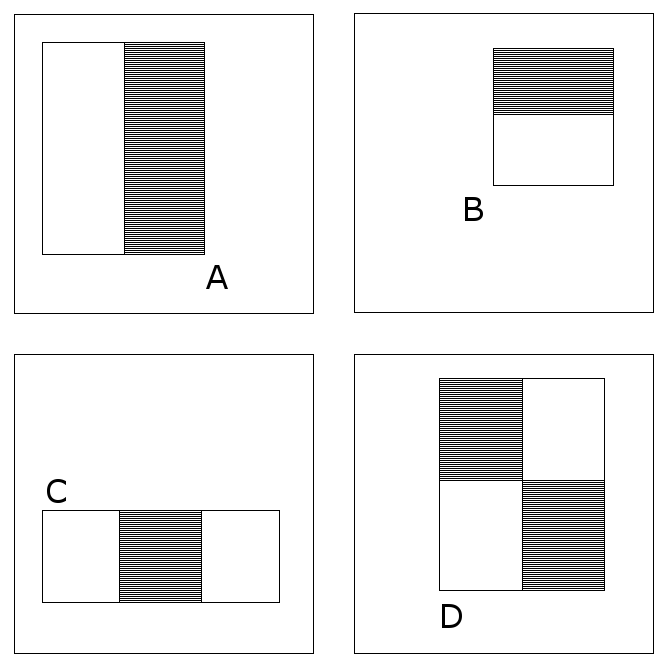
\includegraphics[width=0.5\textwidth]{./haar_features.png}
\caption{Haar-like features used in the Viola-Jones algorithm}
\label{fig:haar_features}
\end{figure}
By using integral images, rectangular features can be evaluated in constant time, obtaining in this way a valuable speed-up over their more complex relatives, like steerable filters \cite{steerable}.
In many applications, however, being able to recognize frontal poses (or "best poses") in a video sequence or in a photo is a fundamental part since it improves drastically the results. For example, if we want to recognize a user, by comparing his face with a database of previously acquired faces, we need to have them in similar poses.
Our aim is to construct a system which is able to better detect frontal poses of a single person in a video source. This is based on geometrical constraints on facial features.

\section*{Methodology}
Our method is based on two fundamental steps: the first one is the face detection, along with the eyes and the mouth, in a video sequence; the second step is the worst pose rejection based on a series of geometric constraints related to the previously extracted facial features.
\subsection*{Feature Detection}
As already stated, the first phase of the algorithm is to find, in real time, the face, eyes and mouth inside each frame of a video source stream. This is done exploiting the Viola-Jones method implementation of the OpenCV library\footnote{http://opencv.org/}. More in detail we apply the following process steps:
\begin{enumerate}
\item Open a video stream and analyze each single frame
\item Face detection
\item Eyes detection
\item Mouth detection
\end{enumerate} 
\subsection*{Best Pose Selection}
\section*{Results}
\section*{Conclusions}

\begin{thebibliography}{9}

\bibitem{viola2004robust}
Viola, Paul, and Michael J. Jones. \emph{``Robust real-time face detection."} International journal of computer vision 57.2 (2004): 137-154.

\bibitem{papageorgiou}
Papageorgiou, Constantine P., Michael Oren, and Tomaso Poggio. \emph{``A general framework for object detection."} Computer vision, 1998. sixth international conference on. IEEE, 1998.

\bibitem{steerable}
Freeman, William T., and Edward H. Adelson. \emph{``The design and use of steerable filters."} IEEE Transactions on Pattern analysis and machine intelligence 13.9 (1991): 891-906.

\end{thebibliography}
\end{document}